\section{Optimization} \label {chapter:optimization}

\subsection{Performance of different networks}
As described in \cref{chapter:training} different networks with different parameters can be compared to obtain the best parameters. \cref{test_val_error} shows the influence of changing the number of hidden neurons. Because the performance of the network is somewhat random due to initializations each training and validation is done 10 times for each set of parameters. The parameters that were held constant were:

\begin{itemize}
\item Amount of hidden layers = 1
\item Learning rate alpha = 0.1
\item Amount of epochs = 20
\end{itemize}

\begin{figure}[!h]
\begin{center}
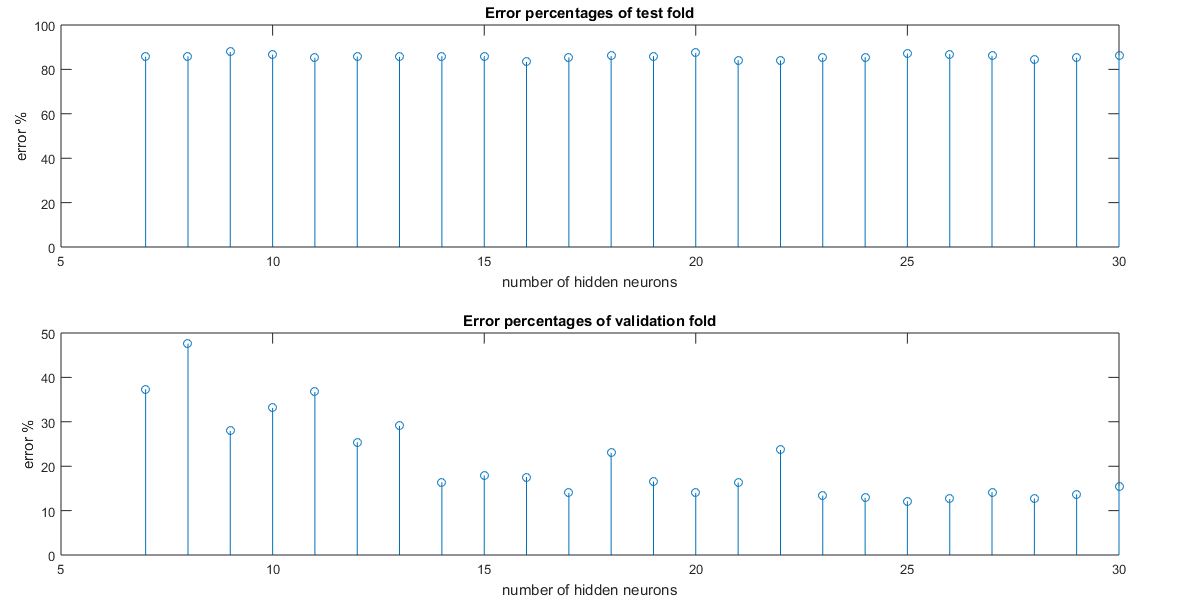
\includegraphics[width=16cm]{testresults/errorpercentages.png}
\caption{Error percentages of test and validation fold }
\label{test_val_error}
\end{center}
\end{figure}
\FloatBarrier

The amount of neurons in the hidden layer is adjusted from 7 to 30 neurons and each time the data for the errors is recorded for 10 runs of the same network. Afterwards the errors of 10 runs are averaged per network and then the errors for the networks are compared with the help of Matlab. \cref{test_val_error} shows that the error percentage definitely decreases with more hidden neurons used, although the relation is not linear and the effect of adding more neurons becomes less and less effective.

\subsection{Optimum parameters}
After many tests, 1 hiddenlayer containing 100 neurons resulted in the lowest stable errorrate. And therefore these parameters are used for determining the outputs of the unknown.txt inputs.


